\documentclass[10pt,a4paper]{standalone}
\usepackage{tikz}
\usetikzlibrary{trees}

\begin{document}
% First, set the overall layout of the tree
% You might need to play with these sizes to ensure nothing overlaps.
\tikzstyle{level 1}=[level distance=1.5cm, sibling distance=2.5cm]
\tikzstyle{level 2}=[level distance=1.5cm, sibling distance=2.5cm]
\tikzstyle{level 3}=[level distance=1.5cm, sibling distance=1cm]
\tikzstyle{level 4}=[level distance=1.5cm, sibling distance=2cm]
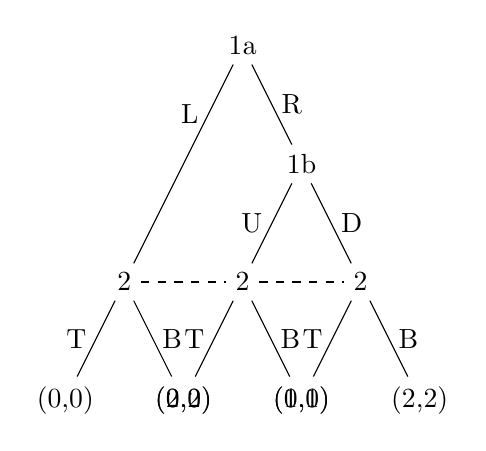
\begin{tikzpicture}
% Start with the parent node, and slowly build out the tree
% with each "child" representing a new level of the diagram
% each "node" represents a labelled (or unlabeled if you
% want) node in the diagram.
\node {1a}
    child{
        child{
                        %Put the name of the node in parenthesis for
                        % reference later. The label shown in the diagram
                        % goes in the brackets. This label can use math mode.
            node(a){2}
            child{
                node{(0,0)}
                                %This allows us to attach a label to the
                                % edge between nodes. This label is just
                                % another node, so we can also name it and
                                % attach things to it.
                edge from parent
                node[left]{T}
            }
            child{
                node{(2,2)}
                edge from parent
                node[right]{B}
            }
                  %Invisible branch to make things align properly.
        } child{edge from parent[draw=none] }
    edge from parent
    node[left]{L}
    }
    child{
        node{1b}
        child{
            node(b){2}
            child{
                node{(0,0)}
                edge from parent
                node[left]{T}
            }
            child{
                node{(0,0)}
                edge from parent
                node[right]{B}
            }
        edge from parent
        node[left]{U}
        }
        child{
            node(c){2}
            child{
                node{(1,1)}
                edge from parent
                node[left]{T}
            }
            child{
                node{(2,2)}
                edge from parent
                node[right]{B}
            }
        edge from parent
        node[right]{D}
        }
    edge from parent
    node[right]{R}
    };
%Now I create the information set. Note that I utilize the names
% that I had previously assigned to nodes in my graph
\draw [dashed](a)--(b);
\draw [dashed](b)--(c);
\end{tikzpicture}
\end{document}